
\documentclass{abgabe}

\begin{document}
\begin{questions}
    \qformat{\thequestion. \textbf{\thequestiontitle} \hfill}
    \titledquestion{Nachrichtenverwaltungssystem}

    Führen Sie die Aufgabe aus dem Praktikum zu Ende.

    Zur Erinnerung:\\
    In einem Nachrichtenverwaltungssystem können sich Kunden für unterschiedliche Nachrichtenkanäle interessieren.
    Dabei kann ein Kunde Nachrichtenkanäle abonnieren und wieder abbestellen.
    Ändert sich ein Nachrichteninhalt eines Nachrichtenkanals, so werden alle Abonnenten (Kunden) unmittelbar informiert.
    Der Kunde kann zwischen verschiedenen Abrechnungsarten für seine Abonnements wählen.
    Für das konkrete Beispiel soll es die Varianten geben, dass für jede Nachricht ein fester Betrag abgerechnet wird und dass man nur jeweils nach jeder dritten Nachricht einen Betrag bezahlen muss.
    Weitere Abrechnungsarten sollen leicht hinzugefügt werden können.

    \begin{parts}
        \part
        Entwerfen Sie ausgehend von den Klassen \texttt{Nachrichtenkanal} und \texttt{Kunde} ein \emph{Klassendiagramm}, das die genannten Forderungen umsetzt.
        Dabei sollen Sie für die Nachrichten und Kunden das Beobachter-Muster (Observer-Observable-Pattern) und das Strategy-Pattern für die Bezahlmethode einsetzen.

        \begin{solution}
            \begin{center}
                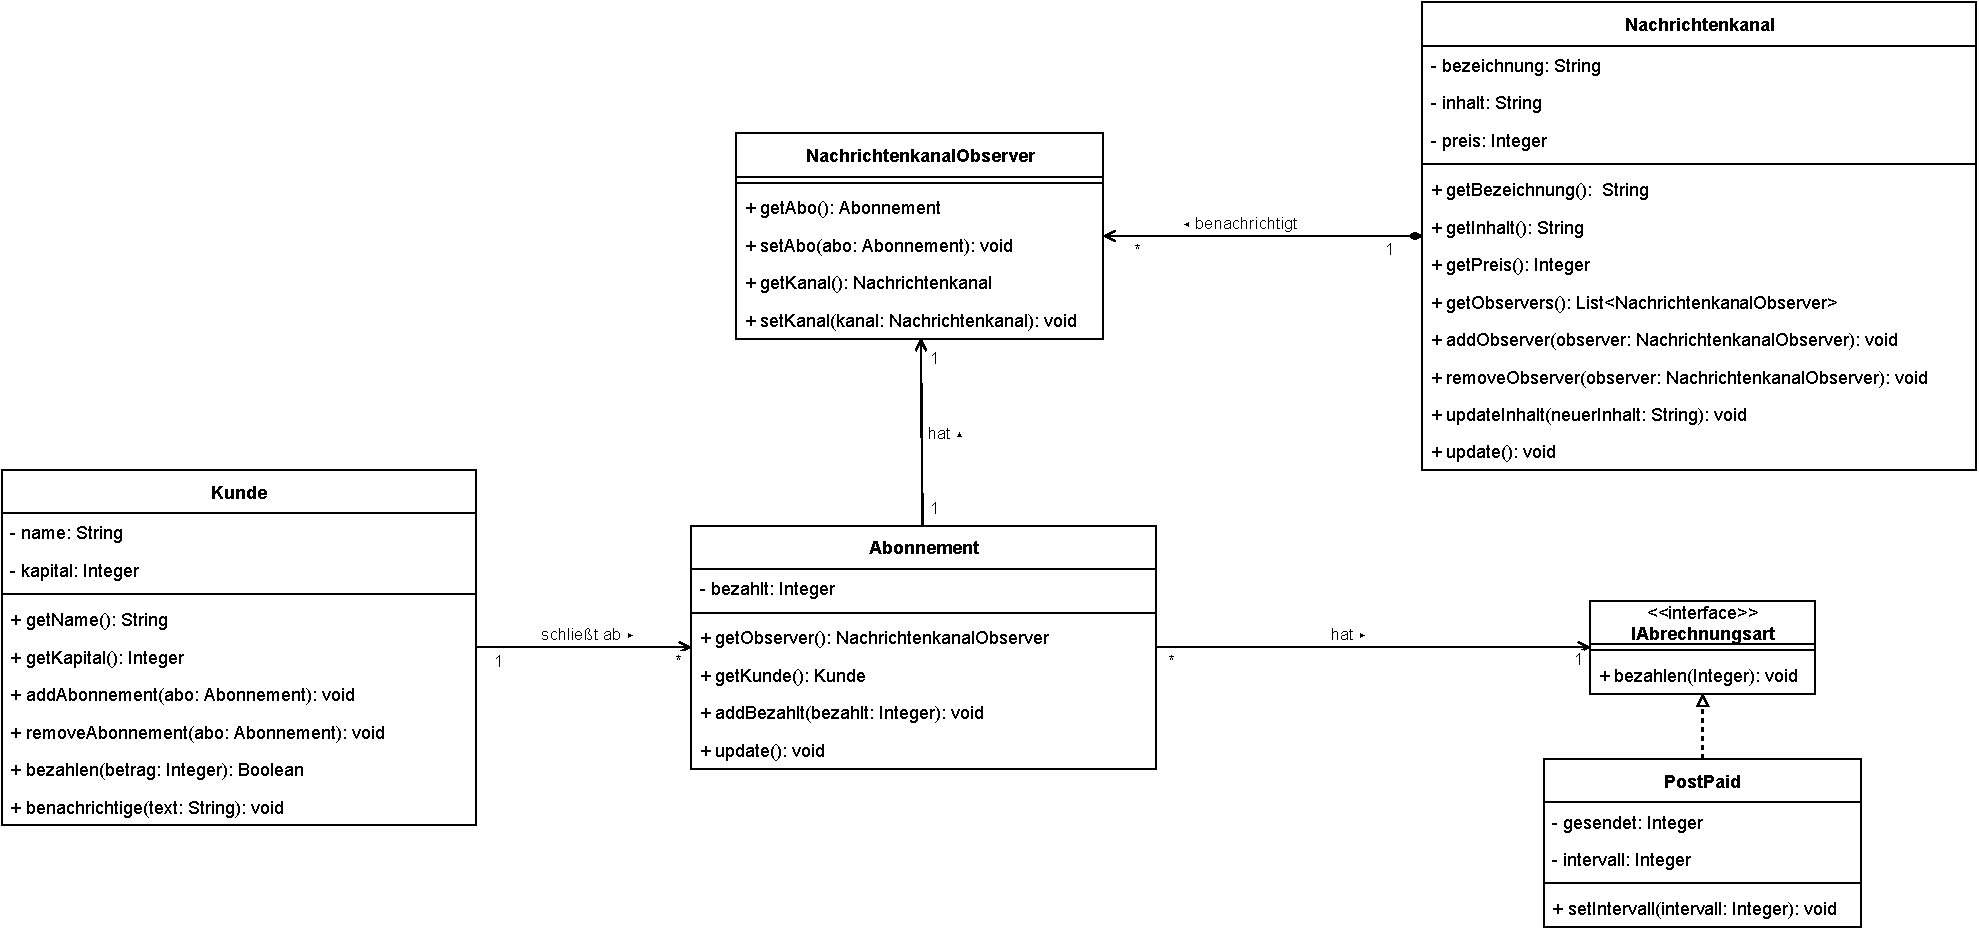
\includegraphics[width=\textwidth]{swt_h08_class.pdf}
            \end{center}
        \end{solution}

        \newpage
        \part
        Geben Sie dann \emph{Implementierungen} aller Klassen an.
        Beachten Sie, dass für versandte Nachrichten eine Abrechnung erfolgen muss.
        Binden Sie den Nutzungsdialog (siehe \texttt{Main.java} und Beispiel-Output) mit ein.
        Mit ihm kann man neue Nachrichten und Kunden anlegen.
        Außerdem kann der Kunden Nachrichtenkanäle mit einer auswählbaren Abrechnungsart wählen und Informationen über alle Nachrichtenkanäle zusammen mit den angefallenen Abokosten anzeigen.
        Natürlich kann man auch die Nachrichteninhalte eines Nachrichtenkanals verändern.
        Der Nutzungsdialog kann nach einigen Schritten wie folgt aussehen, Eingaben sind umrandet
        (Die Datei \texttt{Main.java} sollte entsprechend ergänzt werden).

        \emph{Hinweis: Wie immer ist eine iterative Entwicklung der Lösung sinnvoll, so können Erkenntnisse aus (b) zu Veränderungen der Lösungen von (a) führen!}

        \begin{center}
            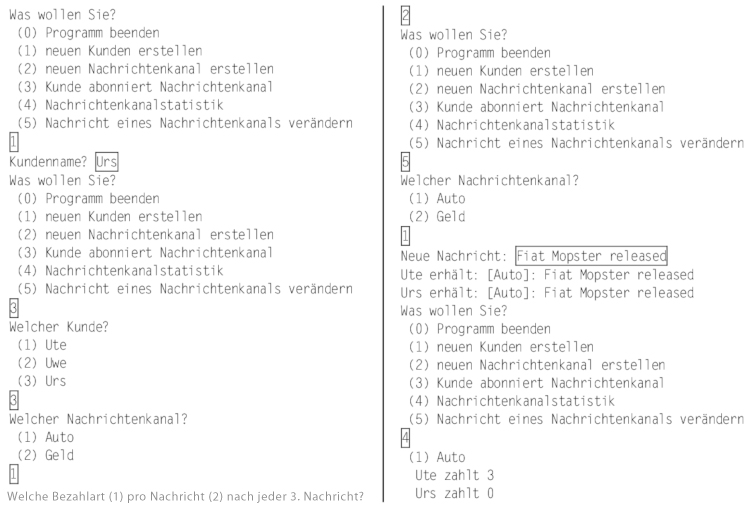
\includegraphics[width=.75\textwidth]{Nachrichtenverwaltungssystem-1_skaliert.jpg}
        \end{center}
        \begin{solution}
            Siehe Anhang.
        \end{solution}
    \end{parts}
\end{questions}

\end{document}